% Pengaturan ukuran teks dan jenis dokumen
\documentclass[11pt]{article}

% Pengaturan ukuran halaman dan margin
\usepackage[a4paper,top=30mm,left=30mm,right=20mm,bottom=20mm]{geometry}

% Pengaturan ukuran spasi
\usepackage[singlespacing]{setspace}

% Judul dokumen
\title{Proposal Pra Tugas Akhir ITS}
\author{Fathullah Auzan Setyo Laksono}

% Pengaturan format bahasa
\usepackage[indonesian]{babel}

% Pengaturan detail pada file PDF
\usepackage[pdfauthor={\@author},bookmarksnumbered,pdfborder={0 0 0}]{hyperref}

% Pengaturan jenis karakter
\usepackage[utf8]{inputenc}

% Pengaturan ukuran indentasi
\setlength{\parindent}{2em}

% Package lainnya
\usepackage{etoolbox} % Mengubah fungsi default
\usepackage{enumitem} % Pembuatan list
\usepackage{lipsum} % Pembuatan template kalimat
\usepackage{graphicx} % Input gambar
\usepackage{longtable} % Pembuatan tabel
\usepackage[table,xcdraw]{xcolor} % Pewarnaan tabel
\usepackage[numbers]{natbib} % Kutipan artikel
\usepackage{changepage} % Pembuatan teks kolom
\usepackage{multicol} % Pembuatan kolom ganda
\usepackage{multirow} % Pembuatan baris ganda
\usepackage{float}
\usepackage{outlines}

% Pengaturan format judul bab
\usepackage{titlesec}
\renewcommand{\thesection}{\arabic{section}}
\titleformat*{\section}{\normalsize\bfseries}
\titleformat*{\subsection}{\normalsize\bfseries}
\titlespacing{\section}{0ex}{3ex}{1.5ex}
\titlespacing{\subsection}{0ex}{3ex}{1.5ex}

% Isi keseluruhan dokumen
\begin{document}

  % Menonaktifkan penomoran halaman
  \pagenumbering{gobble}

  % Lembar pengesahan
  \begin{flushleft}
  % Ubah kalimat berikut sesuai dengan nama departemen dan fakultas
  \textbf{Departemen Teknik Komputer - FTEIC}\\
  \textbf{Institut Teknologi Sepuluh Nopember}\\
\end{flushleft}


\begin{center}
  % Ubah detail mata kuliah berikut sesuai dengan yang ditentukan oleh departemen
  \underline{\textbf{EC184701 - PRA TUGAS AKHIR (2 SKS)}}
\end{center}

\begin{adjustwidth}{-0.2cm}{}
  \begin{tabular}{lcp{0.7\linewidth}}

    % Ubah kalimat-kalimat berikut sesuai dengan nama dan NRP mahasiswa
    Nama Mahasiswa &:& Helmika Mahendra Priyanto \\
    Nomor Pokok &:& 07211840000076\\

    % Ubah kalimat berikut sesuai dengan semester pengajuan proposal
    Semester &:& Ganjil 2021/2022 \\

    % Ubah kalimat-kalimat berikut sesuai dengan nama-nama dosen pembimbing
    Dosen Pembimbing &:& 1. Reza Fuad Rachmadi, S.T., M.T., Ph.D. \\
    & & 2. Dr. Eko Mulyanto Yuniarno, S.T., M.T. \\

    % Ubah kalimat berikut sesuai dengan judul tugas akhir
    Judul Tugas Akhir &:& \textbf{Deteksi Helm Keselamatan Kerja menggunakan CNN} \\

    Uraian Tugas Akhir &:& \\
  \end{tabular}
\end{adjustwidth}

% Ubah paragraf berikut sesuai dengan uraian dari tugas akhir
Keselamatan dan Kesehatan Kerja bertujuan meningkatkan standar dan kualitas kerja 
di era modern ini. Pengaplikasiannya pun beragam, salah satunya yaitu penerapan penggunaan 
helm keselamatan kerja atau helm proyek atau Hard Hat. Medan proyek konstruksi yang berisiko 
tinggi menjadi alasan utama pekerja proyek harus benar - benar mematuhi aturan penggunaan APD, 
dimana salah satunya penggunaan helm proyek. Helm proyek membantu mengurangi dampak benturan 
misal saat pengguna terjatuh atau tertimpa benda berat atau tajam. Tetapi tidak semua personel 
lapangan akan dengan sendirinya mematuhi aturan ini sehingga diperlukannya pengawasan dalam 
penerapan penggunaan helm proyek sebagai salah satu APD keselamatan kerja. Pengawas atau 
supervisor lapangan yang dikerahkan adalah personil manusia yang juga memiliki batasannya 
sebagai manusia. Kondisi lapangan proyek yang luas dan banyaknya personil lapangan akan 
menjadi suatu kesulitan untuk pengawas manusia untuk memastikan tiap personil lapangan 
mematuhi aturan penggunaan helm keselamatan kerja. Maka dari itu, dalam penelitian ini diambil 
suatu tujuan yaitu merancang sistem yang dapat mendeteksi penggunaan helm proyek secara otomatis. Dalam perancangan sistem ini, akan memanfaat Convolutional Neural Network yang didesain untuk rekognisi data dua dimensi. Sistem yang sudah jadi akan diuji pada lapangan proyek konstruksi.
\vspace{1ex}

\begin{flushright}
  % Ubah kalimat berikut sesuai dengan tempat, bulan, dan tahun penulisan
  Surabaya, 9 Desember 2021
\end{flushright}
\vspace{1ex}

\begin{center}

  \begin{multicols}{2}

    Dosen Pembimbing 1
    \vspace{12ex}

    % Ubah kalimat-kalimat berikut sesuai dengan nama dan NIP dosen pembimbing pertama
    \underline{[Reza Fuad Rachmadi, S.T., M.T., Ph.D.]} \\
    NIP. 198504032012121000

    \columnbreak

    Dosen Pembimbing 2
    \vspace{12ex}

    % Ubah kalimat-kalimat berikut sesuai dengan nama dan NIP dosen pembimbing kedua
    \underline{[Dr.Supeno Mardi Susiki Nugroho ST., M.T.]} \\
    NIP. 197003131995121001

  \end{multicols}
  \vspace{6ex}

  Mengetahui, \\
  % Ubah kalimat berikut sesuai dengan jabatan kepala departemen
  Kepala Departemen Teknik Komputer FTEIC - ITS
  \vspace{12ex}

  % Ubah kalimat-kalimat berikut sesuai dengan nama dan NIP kepala departemen
  \underline{Dr. Supeno Mardi Susiki Nugroho, S.T., M.T.} \\
  NIP. 197003131995121001

\end{center}
  \newpage

  \begin{center}
    % Ubah judul
    \textbf{Convolutional Neural Network untuk Estimasi Umur, Gender dan Etnik Berbasis Citra Wajah}
  \end{center}

  % Konten pendahuluan
  \section{PENDAHULUAN}
\label{chap:pendahuluan}

% Ubah bagian-bagian berikut dengan isi dari pendahuluan

Dalam bab ini akan dibahas latar belakang, permasalahan, tujuan, serta batasan masalah pada penelitian ini.

\subsection{Latar Belakang}
\label{sec:latarbelakang}

Keselamatan dan Kesehatan Kerja atau biasa disingkat K3 menjadi usaha untuk meningkatkan kualitas lingkungan kerja agar menjadi lebih aman dan sehat bagi segala pihak yang ada di lingkungan tersebut. Aman dan sehat bisa dalam artian bebas dari kecelakaan, kebakaran, ledakan, lingkungan tercemar, atau wabah penyakit. Tentu saja hal - hal tersebut perlu dihindari karena dapat memberikan dampak kerugian material dan bahkan melayangnya nyawa manusia. Aturan K3 sendiri diatur dalam bentuk norma oleh regulasi pemerintah Republik Indonesia lewat UUD 1945 pasal 27 ayat 2 tentang filosofi penghidupan yang layak, UU No 1 tahun 1970 tentang keselamatan kerja, Undang-Undang No. 13 Tahun 2003 pasal 86 dan 87 Kewajiban penerapan Sistem Manajemen Keselamatan dan Kesehatan Kerja (SMK3), Peraturan Pemerintah No.50 Tahun 2012 tentang Sistem Manajemen Keselamatan dan Kesehatan Kerja (SMK3), dan peraturan pelaksanaan lainnya dari Permenaker, Instruksi Menteri, Pekmenaker.  \cite{ahlik3umum-k3indonesia_2021}
Medan dari proyek konstruksi dapat dianggap sebagai lingkungan yang penuh dengan resiko menjadikannya suatu hal yang patut dipertimbangkan. Bukan hal yang jarang dimana para personel lapangan yang bekerja di suatu proyek konstruksi mengalami cedera akibat hal - hal tertentu. Mulai dari debu konstruksi, puing - puing berterbangan, jatuh dari ketinggian, atau tertimpa benda. Cedera kepala oleh jatuh ketinggian atau tertimpa benda dapat berakibat fatal pada nyawa personil lapangan. \cite{li2020deep}
Helm keselamatan kerja atau \emph{Hardhat} dalam Bahasa inggris atau juga kadang disebut Helm proyek merupakan salah satu bentuk APD K3 yang berfungsi untuk melindungi kepala pengguna dari benturan. Bentuk benturan contohnya kejatuhan benda tajam atau berat yang sekiranya jika tidak menggunakan pelindung akan berdampak fatal pada kepala personil proyek. Selain benturan, helm juga digunakan untuk melindungi kepala penggunanya dari percikan api dan berbagai bentuk serpihan terbang yang biasa ada di lokasi kerja.\cite{k3_mutiaramutu}
Adanya aturan penggunaan helm di suatu proyek konstruksi dengan dasar K3 belum tentu menjamin penggunaan efektif dari helm proyek tersebut. 
Berdasarkan Data Kecelakaan dan Penyakit Akibat Kerja Triwulan II 2020 dari Kemnaker, kecelakaan kerja Tipe A yang meliputi "Terbentur pada umumnya menunjukan kontak atau persinggungan dengan benda tajam atau benda keras yang menyebabkan tergores, terpotong, tertusuk dll" mencapai angka 878 kecelakaan dimana menjadi angka terbesar dibanding tipe kecelakaan lain dengan Tipe J (lain-lain) dengan angka 637 dan Tipe C (terjepit) dengan angka 439 \cite{satudata_kecelakaan_kerja}.
Pengawasan terhadap penerapan Keselamatan Kesehatan Kerja pada suatu proyek seperti menggunakan helm Hard Hat secara konvensional sudah sering dilakukan. Personil pengawas yang dikerahkan untuk memastikan para pekerja di suatu proyek mematuhi aturan keselamatan kerja. Misalnya pengawas ditugaskan untuk mengingatkan pekerja proyek yang tidak menggunakan helm proyek dengan tepat atau bahkan tidak digunakan sama sekali.\cite{li2020deep}

\subsection{Permasalahan}
\label{sec:permasalahan}

Disebutkan pada latar belakang bahwa pengawasan konvensional menggunakan personel manusia untuk menjadi pengawas akan penggunaan helm proyek sebagai APD Keselamatan dan Kesehatan Kerja. Tetapi, teruntuk lokasi proyek konstruksi yang luas dan dengan jumlah pekerja proyek yang banyak menjadikan pengawasan hal yang sulit untuk dilakukan oleh pengawas atau supervisor manusia. Maka dari itu ditarik permasalahan yaitu perlu adanya metode efektif untuk melakukan pengawasan terhadap penggunaan helm proyek secara otomatis. 

\subsection{Tujuan}
\label{sec:Tujuan}

Dari permasalahan yang disebutkan, dapat dapat ditentukan tujuan :

\begin{enumerate}[nolistsep]

  \item Merancang sistem yang dapat mendeteksi pekerja proyek yang menggunakan helm proyek dan yang tidak menggunakan helm proyek secara otomatis
  \item Memicu alarm jika terdeteksi adanya personnel yang tidak menggunakan helm keselamatan kerja dengan benar.

\end{enumerate}

\subsection{Batasan Masalah}
\label{sec:batasanmasalah}

Batasan-batasan dari pengembangan Deteksi Helm Keselmatan Kerja menggunakan CNN meliputi hal - hal berikut:

\begin{enumerate}[nolistsep]

  \item Diasumsikan sistem pengawasan diletakkan pada \emph{checkpoint} masuk kawasan konstruksi

  \item Metode deteksi penggunaan helm keselematan kerja yang akan digunakan pada penelitian ini adalah \emph{You Only Look Once} (YOLO) versi 5 atau YOLOv5.

  \item Jenis input yang akan digunakan untuk deteksi adalah input dari kamera yang diletakkan pada checkpoint masuk kawasan konstruksi.
  \item Sistem hanya mendeteksi "kepala menggunakan helm" dan "kepala yang tidak mengenakan helm".

\end{enumerate}

\subsection{Penelitian Terkait}
\begin{enumerate}
  \item Deep Learning Based Safety Helmet Detection in Engineering Management Based on Convolutional Neural Networks 
  \par Li dan teman teman pada tahun 2020 melakukan penelitian tentang metode deteksi helm keselamatan kerja secara real time berbasis deep learning pada lokasi konstruksi. Li dan teman – teman menggunakan SSD-MobileNet yang berbasis dari CNN. Menggunakan dataset yang berjumlah 3261 gambar helm keselamatan. SSD- Mobilenet dipilih dibanding R-CNN dengan maksud pendeteksian yang lebih cepat dan cocok untuk real – time walau tidak seakurat R-CNN. \cite{li2020deep}
  
  \item Deteksi Penggunaan Helm Pada Pengendara Bermotor Berbasis Deep Learning 
  \par Yusuf Umar pada tahun 2020 melakukan penelitian tentang deteksi penggunaan helm pada pengendara bermotor. Pada penelitiannya menggunakan YOLOv3 yang berbasis dari CNN. Pada sistem yang dikembangkan dapat memberikan bounding box ke pengendara lalu dalam bounding box pengendara terdapat boundbox lain dari kepala hingga dada pengendara untuk mendeteksi penggunaan helm motor ada atau tidak. \cite{hanafi2020deteksi}
\end{enumerate}

\subsection{Gap Penelitian}
Pada penelitian Deep Learning-Based Safety Helmet Detection in Engineering Management Based on Convolutional Neural Networks oleh Li dan kawan - kawan , pendeteksian hanya mendeteksi helm keselamatannya sendiri tetapi belum mendeteksi personel yang tidak menggunakan helm keselamatan. Selain itu, Li dan kawan - kawan tidak menggunakan YOLO dalam penelitiannya dan memilih menggunakan SSD-MobileNet.
\par Pada penelitian Deteksi Penggunaan Helm Pada Pengendara Bermotor Berbasis Deep Learning oleh Yusuf Umar hanya diimplementasikan pada deteksi helm pada pengendara bermotor dan belum untuk helm proyek. Sekiranya metode yang akan digunakan untuk pengembangan sama tetapi dataset yang digunakan akan berbeda.

% \section{Sistematika Penulisan}
% \label{sec:sistematikapenulisan}

% Untuk laporan penelititan pada tugas akhir ini akan disusun dalam beberapa poin yaitu :

% \begin{enumerate}[nolistsep]

%   \item \textbf{BAB I Pendahuluan}

%   Bab ini berisi penjelasan terkait latar belakang, permasalahan, tujuan, batasan masalah, dan sistematika dari penulisan laporan ini.

%   \vspace{2ex}

%   \item \textbf{BAB II Tinjauan Pustaka}

%   Bab kedua ini menguraikan teori - teori yang menjadi fundamental dari permaslaah yang dibahas.

%   \vspace{2ex}

%   \item \textbf{BAB III Desain dan Implementasi Sistem}

%   Bab ini berisi \lipsum[4][1-5]

%   \vspace{2ex}

%   \item \textbf{BAB IV Pengujian dan Analisa}

%   Bab ini berisi \lipsum[5][1-5]

%   \vspace{2ex}

%   \item \textbf{BAB V Penutup}

%   Bab ini berisi \lipsum[6][1-5]

% \end{enumerate}


  % Konten tinjauan pustaka
  \section{TINJAUAN PUSTAKA}
\label{chap:tinjauanpustaka}

% Ubah bagian-bagian berikut dengan isi dari tinjauan pustaka

% Demi mendukung penelitian ini, \lipsum[1][1-5]

% \section{Roket Luar Angkasa}
% \label{sec:roketluarangkasa}

% % Contoh input gambar
% \begin{figure}[ht]
%   \centering

%   % Ubah dengan nama file gambar dan ukuran yang akan digunakan
%   \includegraphics[scale=0.35]{gambar/roketluarangkasa.jpg}

%   % Ubah dengan keterangan gambar yang diinginkan
%   \caption{Peluncuran roket luar angkasa \emph{Discovery} \citep{roketluarangkasa}.}
%   \label{fig:roketluarangkasa}
% \end{figure}

% Roket luar angkasa merupakan \lipsum[1]

% \emph{Discovery}, Gambar \ref{fig:roketluarangkasa}, merupakan \lipsum[2]

\subsection{Deep Learning}
\label{sec:deeplearning}

Deep Learning sejatinya bagian machine learning yang dimana algoritma nya terinspirasi dari cara kerja jaringan neuron seperti 
halnya jaringan neuron pada otak manusia. Pada deep learning, syaraf atau neuron merupakan perwakilan dari satu fungsi yang 
menyimpan suatu nilai atau value yang dimana neuron - neuron ini berada dalam layer - layer yang dimana antar layer memiliki 
hubungan tertentu. Deep Learning digunakan karena kemampuanya untuk menemukan relasi yang tidak ditemukan antara input dan output. \cite{Goodfellow-et-al-2016}

% \emph{Discovery}, Gambar \ref{fig:roketluarangkasa}, merupakan \lipsum[2]

\subsection{Convolutional Neural Network}
\label{sec:convolutionalneuralnetwork}

Convolutional Neural Network adalah metode deep learning yang didesain untuk rekognisi pada data dua dimensi yang dimana umumnya berupa gambar visual (tetapi tidak harus berupa gambar) dan untuk klasifikasi. Deep Learning dapat mengatasi masalah dimana terdapat terlalu banyak parameter.  Layer yang biasanya ada di dalam CNN yaitu input layer, convolutional layer, activation layer, dan fully connected layer.
Convolutional layer dan pooling layer merupakan bagian utama pada CNN. Layer - layer tersebut dapat menemukan karakteristik dari objek. Convolutional layer memiliki kapabilitas untuk menemukan dan meningkatkan fitur/karakteristik objek sedangkan pooling layer mampu menyaring fitur fitur yang ditemukan dengan menghapus layer yang tidak diperlukan atau meng-compress fitur. Activation layer memanfaatkan aktivasi non linear untuk meningkatkan expression ability dari model neural network. Fully Connected layer berfungsi untuk menggabungkan fitur - fitur objek dengan nilai output fitur. \cite{Goodfellow-et-al-2016}

% \subsection{Hukum Newton}
% \label{subsec:hukumnewton}

% Newton \citep{newton1687} pernah merumuskan bahwa \lipsum[1]
% Kemudian menjadi persamaan seperti pada persamaan \ref{eq:hukumpertamanewton}.

% % Contoh pembuatan persamaan
% \begin{equation}
%   \label{eq:hukumpertamanewton}
%   \sum \mathbf{F} = 0\; \Leftrightarrow\; \frac{\mathrm{d} \mathbf{v} }{\mathrm{d}t} = 0.
% \end{equation}

% \subsection{Anti Gravitasi}
% \label{subsec:antigravitasi}

% Anti gravitasi merupakan \lipsum[1]


\subsection{Visi Komputer}
\label{sec:visikomputer}

Convolutional Neural Network adalah metode deep learning yang didesain untuk rekognisi pada data dua dimensi yang dimana umumnya berupa gambar visual (tetapi tidak harus berupa gambar) dan untuk klasifikasi. Deep Learning dapat mengatasi masalah dimana terdapat terlalu banyak parameter.  Layer yang biasanya ada di dalam CNN yaitu input layer, convolutional layer, activation layer, dan fully connected layer.
Convolutional layer dan pooling layer merupakan bagian utama pada CNN. Layer - layer tersebut dapat menemukan karakteristik dari objek. Convolutional layer memiliki kapabilitas untuk menemukan dan meningkatkan fitur/karakteristik objek sedangkan pooling layer mampu menyaring fitur fitur yang ditemukan dengan menghapus layer yang tidak diperlukan atau meng-compress fitur. Activation layer memanfaatkan aktivasi non linear untuk meningkatkan expression ability dari model neural network. Fully Connected layer berfungsi untuk menggabungkan fitur - fitur objek dengan nilai output fitur. \cite{Goodfellow-et-al-2016}

\subsection{You Only Look Once (YOLO)}
\label{sec:youonlylookone}

You Only Look Once adalah algoritma yang memiliki kemampuan untuk mendeteksi dan mengenal 
objek yang ada di suatu gambar yang dimana hanya memerlukan satu propagasi di neural network. 
YOLO menggunakan CNN untuk melakukan deteksi objek secara real time. 
Dengan menggunakan YOLO berarti untuk melakukan deteksi pada suatu gambar hanya memerlukan 
sekali run .\cite{adiwibowo2020deteksi}


\subsection{Helm Keselamatan Kerja}
\label{sec:helmkeselamatankerja}

Helm Keselamatan Kerja atau yang kadang disebut Helm Proyek atau Hardhat  dalam bahasa inggris berfungsi sebagaimana helm pada umumnya berfungsi yaitu untuk melindungi kepala penggunanya. Berbeda dengan helm lainnya seperti helm motor atau helm militer, helm proyek digunakan umumnya pada proyek konstruksi untuk melindungi pekerja dari hantaman ke kepala saat terjatuh atau tertimpa benda berat yang dimana sering terjadi di wilayah konstruksi. \cite{safeopedia_2018}

  % Konten metodologi
  \section{METODOLOGI}
\label{chap:desainimplementasi}

% Ubah bagian-bagian berikut dengan isi dari desain dan implementasi

% Penelitian ini dilaksanakan sesuai \lipsum[1][1-5]

\subsection{Data dan Peralatan / Data dan Alat Bantu / Material}
\label{sec:perlengkapan}


\begin{enumerate}
  \item Dataset
  \par \emph{Dataset} yang digunakan yaitu gambar atau foto yang meliputi gambar personel atau manusia yang menggunaka helm keselamatan kerja dan/atau manusia yang tidak menggunakan helm keselamatan kerja.
  Selama penulisan proposal ini, dataset yang sudah didapatkan yaitu :
  \begin{enumerate}
    \item \emph{Safety helmet detection} oleh andrewmvd
    \par Dataset ini berisi 5000 gambar pekerja konstruksi yang meliputi orang yang menggunakan helm dan yang tidak menggunakan helm keselamatan kerja. Masin - masing gambar sudah diberi label
    \emph{"helmet"} dan \emph{"head"}. Format anotasi label nya berupa fromat PASCAL VOC yang disimpan dalam file .xml.
  \end{enumerate}
  \par Kedepannya akan dilakukan pengumpulan lebih untuk dataset.

  \item Alat Bantu
  \begin{enumerate}
    \item Anaconda
    \par Anaconda sendiri merupakan package distribution yang dibuat khusus untuk data science. Anaconda biasanya digunakan untuk membuat environment baru untuk mengisolasi proyek dan menginstall package untuk keperluan tertentu. Pada penelitian ini akan digunakan untuk membantu penulis dalam mengumpulkan package - package yang diperlukan untuk melakukan proses training dan pengembangan sistem.\cite{pankajmathur_2018}

    \item Python 3.7
    \par Python sendiri adalah bahasa pemrograman high level yang sudah terinterpretasi dan berbasis objek. Struktur data yang sudah ada di dalam python dan penulisan syntax yang sederhana dan mudah dipahami dapat meningkatkan performa pengerjaan. Pada penelitian ini python digunakan karena merupakan bahasa pemrograman yang cocok untuk data science mengingat struktur data di python yang dinamis. Selain itu python juga sudah termasuk saat menginstall Anaconda \cite{python.org}

    \item Visual Studio Code
    \par Visual Studio Code adalah source code editor yang ramah performa dan mudah digunakan untuk segala bentuk keperluan penulisan text sehari - harinya. Visual Code mendukung banyak bahasa pemrograman dan menyediakan fitur addons yang digunakan untuk mendownload package untuk berbagai macam kebutuhan berbeda. Pada penelitian ini Visual Studio Code digunakan untuk menulisa script python yang akan digunakan untuk training, pengembangan sistem, dan keperluan lainyna yang sekiranya dibutuhkan pada penelitian ini dan dapat diselesaikan dengan visual studio code.\cite{microsoft_2021}

    \item Roboflow
    \par Roboflow merupakan \emph{tools} yang membantu developer untuk mengolah segala keperluan untuk melakukan pengembangan di bidang visi komputer. Fasilitas yang ditawarkan oleh Roboflow meliputi : pengorganisasian dataset, 
    pelabelan atau \emph{annotation} , pembagian rasio \emph{train/test}, \emph{preprocessing} yang meliputi re-size ukuran gambar, isolasi objek, grayscale, auto-adjust contrast, tile, dan bahkan sekaligus train. 

  \end{enumerate}


\end{enumerate}



\subsection{Metodologi Penelitian}
\label{metodologipenelitian}

\begin{figure}[ht]
  \centering
  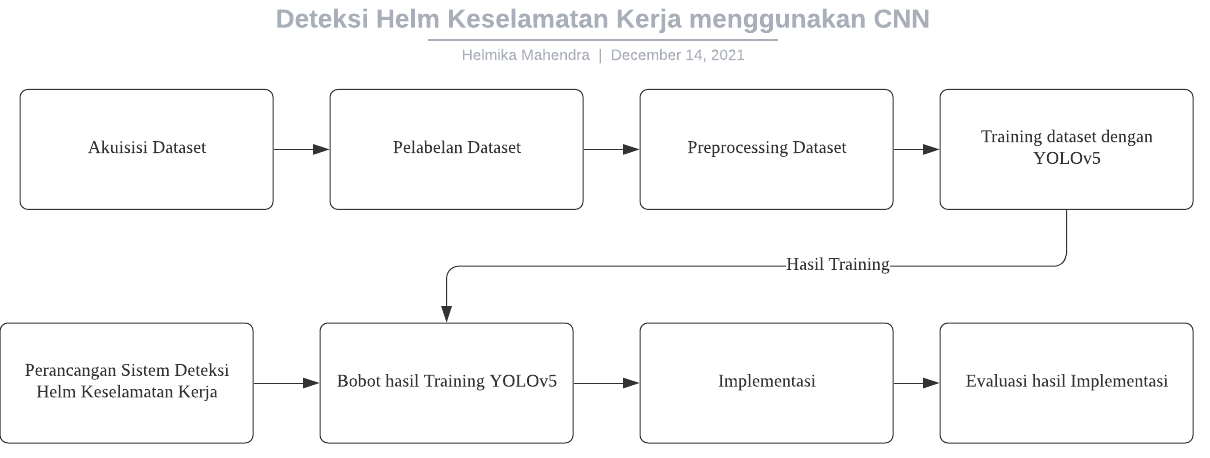
\includegraphics[scale=0.7]{gambar/Metodologi CNN.png}
  \caption{Block Diagram Penelitian Deteksi Helm Keselamatan kerja Menggunakan CNN}
  \label{fig:blockdiagramhelmetdetection}  
\end{figure}

\begin{enumerate}
  \item Akuisisi Dataset
  \par Dibutuhkan kumpulan gambar yang digunakan sebagai \emph{dataset} untuk melakukan \emph{training} dengan YOLOv5 untuk menghasilkan bobot yang lalu digunakan untuk melakukan 
  deteksi personel yang menggunakan helm keselamatan kerja dan pengguna yang tidak menggunakan helm keselamatan kerja. Gambar yang akan digunakan perlu meliputi kepala manusia tanpa helm atau
  kepala manusia yang mengenakan helm. Dibutuhkan berbagai variasi untuk tiap ketentuan baik yang mengenakan helm dan yang tidak mengenakan helm dengan harapan akan meningkatkan kemampuan
  prediksi pada saat diimplementasikan pada sistem seperti variasi dari jauh dekat, warna helm, keadaan cuaca atau pencayaannya.
  \par Metode pengumpulan atau akuisisi dataset nya meliputi pencarian atau \emph{browsing} gambar di internet, mengambil dataset yang digunakan oleh penilitian terkait, dan membuat sendiri dari foto
  menggunakan helm keselamatan kerja.

  \item Pelabelan Dataset
  \par Gambar - gambar yang sudah dikumpulkan dan dijadikan dataset perlu diberi pelabelan untuk masing - masing kelas atau label. Pada penelitian ini, label yang dibuat berjumlah 2 yaitu 
  "head" dan "helmet". Pemberian bounding box untuk label \emph{"head"} meliputi dari ujung kepala (rambut) hingga leher dan untuk label \emph{"helmet"} meliputi seluruh bagian helm 
  keselamatan kerja hingga leher. Untuk penelitian ini, helm yang akan dideteksi sebagai label "helm" yaitu helm keselamatan kerja. Anotasi dari pelabelan akan disimpan kedalam format yang diterima oleh YOLOv5 yaitu format PyTorch yang disimpan dalam file .txt dan .yaml untuk \emph{config}.
  Proses pelabelan pada gambar hanya dilakukan pada gambar atau dataset yang belum memiliki pelabelan. Pada dataset yang sudah didapatkan pada penulisan proposal ini, \emph{Safety helmet detection} oleh andrewmvd, sudah memiliki
  pelabelan.
  \par Pelabelan dilakukan menggunakan Roboflow menggunakan fitur \emph{Annotate}. Fitur \emph{Annotate} dari Roboflow memberikan kemudahan ke pengguna dimana pengguna hanya perlu men-drag bounding
  box di area yang akan diberi label dan memilih kelas labelnya. 
  
  \item Preprocessing Dataset
  \par Sebelum dapat digunakan untuk training menggunakan YOLOv5, perlu dilakukan beberapa modifikasi pada dataset yang sudah dikumpulkan. Hal ini dilakukan untuk menyesuaikan konfigurasi 
  yang ditentukan untuk train dan detect. Proses ini meliputi pengaturan rasio jumlah gambar untuk train-test-validation dan re-size gambar.
  \par Pengaturan rasio jumlah gambar untuk train-test-validation dilakukan di Roboflow pada bagian Generate New Version dari dataset yang sudah di upload ke Roboflow. Pada penilitian ini akan dilakukan beberapa percobaan untuk rasio dataset yang akan menghasilkan hasil bobot yang paling bagus.
  \par Pengaturan ukuran gambar akan disesuaikan dengan hardware yang akan digunakan untuk melakukan training menggunakan YOLOv5. Roboflow juga menyediakan fitur \emph{re-size} untuk mengatur ulang
  ukuran gambar.
  \par Setelah melakukan pemrosesan, Roboflow memberikan fitur export yang akan mengoutputkan \emph{command line} untuk download. \emph{Command line} juga disesuaikan untuk versi \emph{pre-processing} yang disimpan
  di Roboflow.

  \item Training Dataset dan Validasi
  \par Untuk melakukan training dataset, digunakan source code yang sudah diberikan dari repository YOLOv5 oleh Glenn Jocher. Dalam melakukan training akan dilakukan beberapa training menggunakan model yang sudah disediakan
  dari YOLOv5 seperti YOLOv5s, YOLOv5m, YOLOv5l, dan YOLOv5x. Bobot yang dihasilkan dari masing - masing training menggunakan model yang berbeda akan dibandingkan \emph{metrics}-nya seperti precision, recall, dan mAP. Format bobot yang dihasilkan
  dari training menggunakan YOLOv5 akan berupa .pt yang nanti bisa dicoba menggunakan source code detect.py yang disediakan juga dari repo YOLOv5.
  Proses training akan dilakukan di hardware milik penulis dan/atau menggunakan \emph{Google Colab}.

  \item Pengembangan Sistem
  \par Perlu dilakukannya pengembangan sistem yang dapat menerima input video real time dari kamera yang lalu dapat melakukan identifikasi penggunaan helm dan tidak yang dimana dilakukan
  dengan menggunakan model yang sudah dibuat. Sistem yang akan menajalankan bobot yang dihasilkan dari training menggunakan YOLOv5 akan dikembangkan dengan asumsi :
  \begin{enumerate}
    \item Jenis input yang akan digunakan untuk deteksi oleh sistem adalah \emph{live-feed} dari kamera.
    \item Kamera yang digunakan untuk mengawasi diletakkan pada checkpoint masuk ke lokasi utama konstruksi dimana outlet listrik umumnya ada pada suatu lokasi konstruksi.
    \item Sistem akan dijalankan pada suatu komputer yang berada di lokasi konstruksi.
    \item Sistem akan memicu atau men-\emph{trigger} suatu mekanisme alarm.
  \end{enumerate} 

  \item Implementasi
  \par Sistem yang selesai dikembangkan akan diimplementasikan untuk melakukan deteksi pada manusia yang menggunakan helm dan yang tidak dengan input dari kamera atau web cam yang mengirimkan input live-feed.
  Implementasinya juga akan dilakukan pada lokasi konstruksi nyata jika memungkinkan.

  \item Pengujian dan Evaluasi
  \par Dari proses implementasi akan dilakukan pengujian keberhasilan dan keefektifan sistem saat dikerahkan pada implementasi dunia nyata.

\end{enumerate}


% % Contoh pembuatan potongan kode
% \begin{lstlisting}[
%   language=C++,
%   caption={Program halo dunia.},
%   label={lst:halodunia}
% ]
% #include <iostream>

% int main() {
%     std::cout << "Halo Dunia!";
%     return 0;
% }
% \end{lstlisting}

% \lipsum[2-3]

% % Contoh input potongan kode dari file
% \lstinputlisting[
%   language=Python,
%   caption={Program perhitungan bilangan prima.},
%   label={lst:bilanganprima}
% ]{program/bilangan-prima.py}

% \lipsum[4]


  % Konten lainnya
  \section{HASIL YANG DIHARAPKAN}

Pada akhir pengembangan diharapkan dihasilkan sistem yang dapat membedakan dan mendeteksi personil lapangan yang menggunakan helm dan tidak menggunakan helm secara otomatis dan real-time dan akan
memicu mekanisme alarm jika terdeteksi personel yang tidak menggunakan helm proyek.


\section{RENCANA KERJA}

% Ubah tabel berikut sesuai dengan isi dari rencana kerja
\newcommand{\w}{}
\newcommand{\G}{\cellcolor{gray}}
\begin{table}[h!]
  \begin{tabular}{|p{3.5cm}|c|c|c|c|c|c|c|c|c|c|c|c|c|c|c|c|}

    \hline
    \multirow{2}{*}{Kegiatan} & \multicolumn{16}{|c|}{Minggu} \\
    \cline{2-17} &
    1 & 2 & 3 & 4 & 5 & 6 & 7 & 8 & 9 & 10 & 11 & 12 & 13 & 14 & 15 & 16 \\
    \hline

    % Gunakan \G untuk mengisi sel dan \w untuk mengosongkan sel
    Studi Literatur &
    \G & \G & \G & \G & \G & \w & \w & \w & \w & \w & \w & \w & \w & \w & \w & \w \\
    \hline

    Pembuatan Model &
    \w & \w & \w & \G & \G & \G & \G & \G & \w & \w & \w & \w & \w & \w & \w & \w \\
    \hline

    Perancangan Sistem &
    \w & \w & \w & \w & \w & \w & \G & \G & \G & \G & \G & \w & \w & \w & \w & \w \\
    \hline

    Implementasi dan Evaluasi &
    \w & \w & \w & \w & \w & \w & \w & \w & \w & \w & \w & \G & \w & \w & \w & \w \\
    \hline
    
    Penulisan Laporan &
    \w & \w & \w & \w & \w & \w & \w & \w & \w & \w & \w & \w & \G & \G & \G & \G \\
    \hline

  \end{tabular}
\end{table}

  % Daftar pustaka
  \renewcommand\bibname{DAFTAR PUSTAKA}
  \addcontentsline{toc}{chapter}{\bibname}
  \bibliographystyle{unsrtnat}
  \bibliography{dafpus/pustaka.bib}
  \cleardoublepage
  %\section{DAFTAR PUSTAKA}
  %\renewcommand\refname{}
  %\vspace{-2ex}
  %\bibliographystyle{unsrtnat}
  %\bibliography{pustaka/pustaka.bib}

\end{document}